\section{Discussion}

% \todo{Suggest try and strucuture this a bit more e.g. each para bold the key lesson @ start of para. Can you group into implications for research/implications for practice to make more actionable??}

This paper presents the interactive type debugging tool \chameleon{} and charts the evolution of its design across several iterations in response to user evaluation and feedback, as well as examines   the effectiveness of the general approach compared to traditional static type error messages. We found that programmers using \chameleon{} are able to debug errors faster than using traditional text-based error messages. This effect is shown more clearly when the task is not trivial. We found that programmers who actively use \chameleon{}'s interactive features are more efficient in fixing type errors than passively reading the type error output. In this section, we will discuss a few interpretations of the results.


\subsection{Effect on Reading Source Code}
From the results of Study 1a, we observed that the choice of debugging tool had little effect on how fast programmers solve simple type errors. Conversely, when facing more realistic problems (longer source code, error locations more scattered) in study 1b, programmers are more effective using \chameleon{}. One explanation is that \chameleon{} reduces the amount of reading time by taking programmers more directly to the problem. Earlier studies \cite{Jbara2015-gr, Peitek2020-nb} showed that reading source code is generally the initial step of solving programming problems and is done in several passes. Although traditional compiler error message tools initially show fewer locations, these may be incomplete, meaning that programmers have to expand the reading span without clear guidance. In contrast, \chameleon{} shows more error locations initially. However, the completeness of error locations assures programmers which part of the source code can be safely skipped.

\subsection{Forming Debugging Plans}
From the results of Study 2, we found that programmers who use the interactive tool fix type errors faster than the ones who passively read the error output. This effect is stronger in harder tasks. We speculate that one factor of this result is that  \chameleon{} helps to develop debugging plans. We observed that when working with \chameleon{}, programmers form different debugging plans to attack the problem. Among the \textit{high} interactivity participants in user study 2, some programmers cycle through deduction steps as a guide to reading source code; some navigate to both ends of the deduction chain where types are normally grounded and concrete. In contrast, \textit{minimal} interactive participants generally form similar plans, including carefully reading the program text and manually annotating expressions based on their understanding of the program.


\subsection{Externalize Intermediate Typing Information}
We speculate another factor of the effectiveness of \chameleon{} interactive debugging tools is that they help programmers effectively chunk intermediate information. With the program shown in Fig.~\ref{fig:listing2}, \chameleon{} offers two candidate expressions: \texttt{f} can be typed as \texttt{Int -> Bool} or \texttt{Char -> Bool}; \texttt{z} can be typed as \texttt{Int} or \texttt{Char}. Although  these two statements are equivalent in theory, programmers are often required to compute the latter from the former or vice versa. And this computation may carry out multiple layers. Programmers have to remember all the intermediate types and their reasoning throughout such mental gymnastics. Assisted by candidate expression cards and deduction steps, this intermediate information is externalized on screen and can be retrieved anytime. A recent study on working memory \cite{Crichton2021-ru} suggested this approach may provide a positive effect in helping programmers manage cognitive load and free up working-memory space for high-level thinking.

% \subsection{Implication for future studies}
% Our study aims to contribute to the wider understanding of program comprehension in the context of advanced type systems. One promising research area to extend our results is to apply the design of \chameleon{} to other languages with high demand for explainability\cite{ferdowsi_usability_2023}.

% Colorization and overlay widgets are used to visualize relations and orders that may not conform to the source code structures. These techniques fit well to types because the introduction and elimination of typing constraints tend to be scattered throughout the program. A interesting question is whether these techniques can also be applied to other program properties, such as memory allocation and freeing, as well as message dispatching and consumption, which also exhibit similar patterns.

% Finally, we employed MUS (minimal unsatisfiable subset) for fault localization and types recovery, but we are also curious about the possibility of further analysis based on MUS to power advanced debugging systems, such as efficient and accurate type error repair by combining our results with mutation testing or solution searching based on machine learning.

\begin{figure}
    \centering
    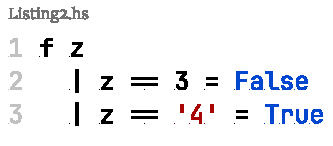
\includegraphics[width=\linewidth]{images/Listing2.pdf}
    \caption{\chameleon{} reports an error in the expressions \texttt{f} and \texttt{z}}
    \label{fig:listing2}
\end{figure}

% \begin{listing}
% \begin{minted}[bgcolor=bg,linenos]{haskell}
% f z     
%     | z == 3 = False
%     | z == '4' = True
% \end{minted}
% \vspace*{-9mm}
% \caption{\chameleon{} reports an error in the expressions \texttt{f} and \texttt{z}}
% \label{listing:2}
% \end{listing}
% Implication for research
% In our studies, \chameleon{} shows a few different designs for type error visualization and interaction. However, we are far from exhausting the search space. One challenge we notice in the current design is that programmers have to shift their focus between the editor on the left and the \chameleon{} debugging interface on the right. Using the hover popup window in most mainstream IDEs may reduce the context switching during debugging.

% Integration with existing tools
% The current implementation of \chameleon{} requires non-trivial adaptation for editors such as VS Code and IntelliJ due to the overlay explanation layer. This type of error visualization is non-standard in mainstream editors. However, there may exist alternative representations of \chameleon{} error reporting using only the features available in major editors and IDEs. It is especially beneficial to represent \chameleon{} errors using a universal debugging middle layer such as language server protocol (LSP). This will allow \chameleon{}  to be adapted into various coding environments which support an LSP back end.


% Extend to other languages
% Our study focuses on the Haskell language for its popularity in the academic world. However, the low quality of textual type errors is a problem not limited to Haskell. Modern statically typed languages more or less all share the same problem. We believe the underlying type reporting technique and algorithms can be generalized to other languages. It will be exciting to see how interactive debugging features perform in other paradigms, such as  imperative languages and incremental type systems.

% Ranking candidate expressions and alternative types
% Our design of \chameleon{}  emphasizes allowing programmers to update the type error based on their prior knowledge. It unfolds to answer three questions: which expression should be considered ill-typed? Between multiple possible types, which one should be considered intended? Among all the possible locations, which one should be considered the cause? \chameleon{} answers all three questions by leaving them to the hands of the programmers. However, it is possible in situations, prescriptive error messages are preferred. Using heuristic methods may achieve the best of both worlds. It may produce effective results by guessing the possible un-typable expression based on the position it appears in the syntax tree and project structure or guessing the intended type signature by comparing the number of supporting slices in the source code.
